\documentclass[border=10pt]{standalone}

\usepackage{tikz}
\usepackage{tikzsymbols}
\usetikzlibrary{calc,patterns,shapes.geometric}

\def\centerarc[#1](#2)(#3:#4:#5){\draw[#1] ($(#2)+({#5*cos(#3)},{#5*sin(#3)})$) arc (#3:#4:#5);}

\begin{document}
	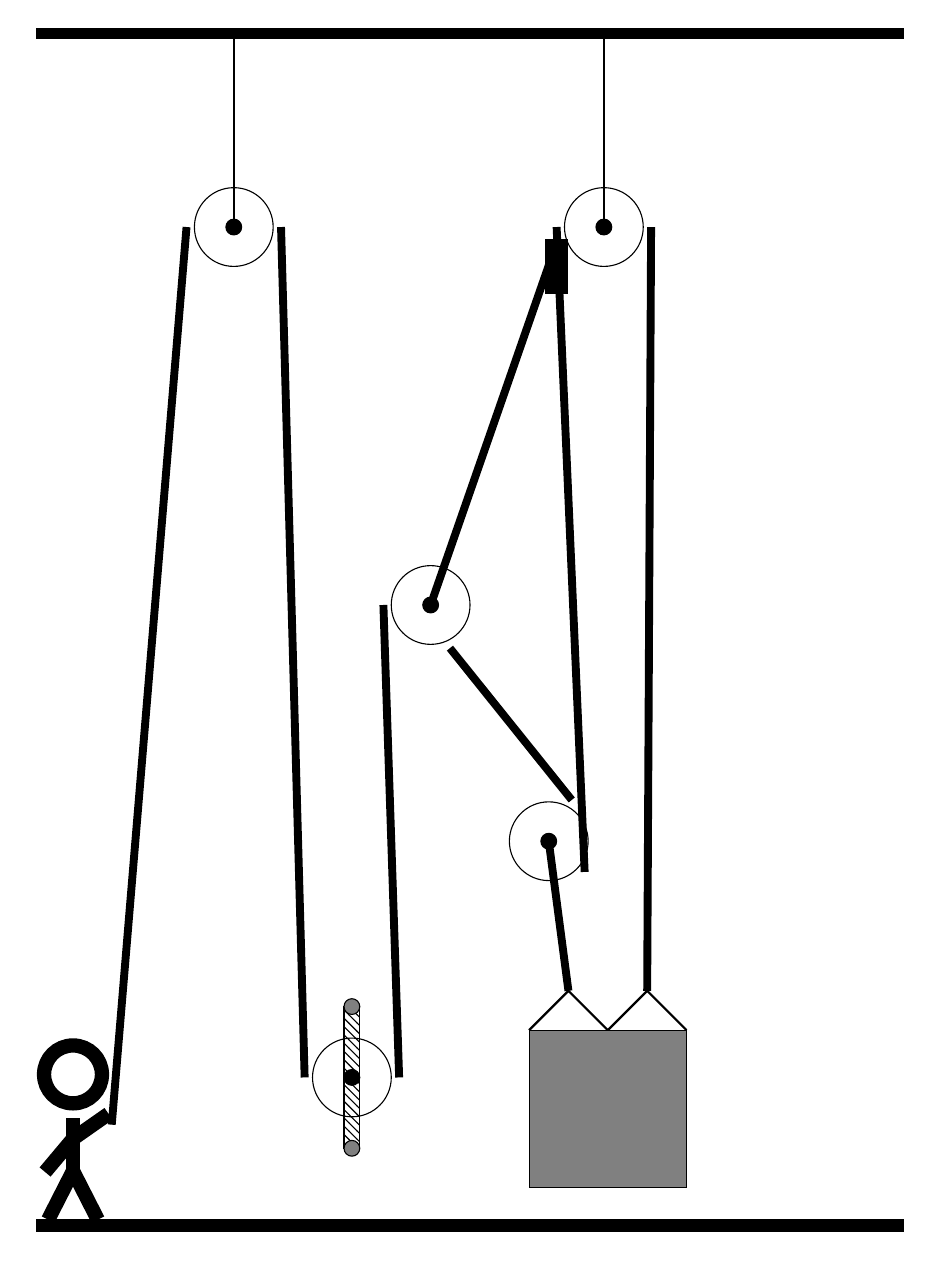
\begin{tikzpicture}
		%%%%% START %%%%%
		\draw[fill=black] (-6, 12) rectangle (5, 12.125);
		
		\draw (-1, 4.8) circle (0.5);
		\draw[fill=black] (-1, 4.8) circle (0.1);
		
		\draw (0.5, 1.8) circle (0.5);
		\draw[fill=black] (0.5, 1.8) circle (0.1);
		
		\draw (1.2, 9.6) circle (0.5);
		\draw[fill=black] (1.2, 9.6) circle (0.1);
		\draw[thick] (1.2, 9.6) -- (1.2, 12);
		
		\draw (-3.5, 9.6) circle (0.5);
		\draw[fill=black] (-3.5, 9.6) circle (0.1);
		\draw[thick] (-3.5, 9.6) -- (-3.5, 12);
		
		\draw (-2, -1.2) circle (0.5);
		\draw[fill=black] (-2, -1.2) circle (0.1);
		\draw[pattern=north west lines, pattern color=black] (-2.1, -0.3) rectangle (-1.9, -2.1);
		\draw[fill=black!50] (-2, -0.3) circle (0.1);
		\draw[fill=black!50] (-2, -2.1) circle (0.1);
		
		\draw[thick]  (0.25, -0.6) -- (0.75, -0.1) -- (1.25, -0.6) -- (1.75, -0.1) -- (2.25, -0.6);
		\draw[fill=black!50] (0.25, -0.6) rectangle (2.25, -2.6);
		\draw[line width=1mm] (-5.05, -1.8) -- (-4.1, 9.6);
		\centerarc[line width=1mm](-3.5, 9.6)(0:180:0.6);
		\draw[line width=1mm] (-2.9, 9.6) -- (-2.6, -1.2);
		\centerarc[line width=1mm](-2, -1.2)(180:360:0.6);
		\draw[line width=1mm] (-1.4, -1.2) -- (-1.6, 4.8);
		\draw[line width=1mm] (-1, 4.8) -- (0.6, 9.4);
		\draw[line width=1mm, fill=black](0.5, 8.8) rectangle (0.7, 9.4);
		\centerarc[line width=1mm](-1, 4.8)(-20:180:0.6);
		\draw[line width=1mm] (-0.755, 4.252) -- (0.792, 2.324);
		\centerarc[line width=1mm](0.5, 1.8)(160:380:0.6);
		\draw[line width=1mm] (0.956, 1.41) -- (0.6, 9.6);
		\draw[line width=1mm](0.5, 1.8) -- (0.75, -0.1);
		\centerarc[line width=1mm](1.2, 9.6)(0:180:0.6);
		\draw[line width=1mm] (1.8, 9.6) -- (1.75, -0.1);
		
		\node at (-5.5, -1.9) {\Strichmaxerl[10][50][35]};
		
		\draw[fill=black] (-6, -3) rectangle (5, -3.15);
		%%%%% END %%%%%
	\end{tikzpicture}
\end{document}